\newpage
\section{Nikodem Jakubowski}
\label{sec:pawljmlo}

\begin{center}
{\Large Dodałem zdjęcie kotka} (patrz Figure~\ref{fig:kotek}).
\end{center}


\begin{figure}[htbp] % Co oznacza [htbp]?
    \centering
    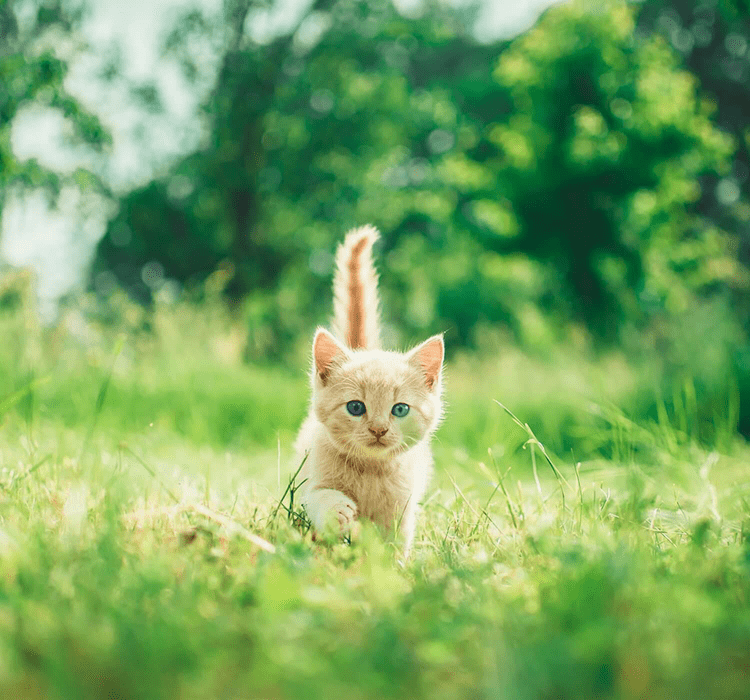
\includegraphics[width=0.8\textwidth]{pictures/kotek.png} % Jak sprawić, żeby obrazek był większy?
    \caption{Ten kotek jest malutki}
    \label{fig:kotek}
\end{figure}

{\Large Tabela~\ref{tab:ranking} to ranking grupy F z LM, 2007r.} % Do czego służy \ref{}?

\begin{table}[htbp]
\centering
\begin{tabular}{l*{6}{c}r}
Team              & P & W & D & L & F  & A & Pts \\
\hline
Manchester United & 6 & 4 & 0 & 2 & 10 & 5 & 12  \\
Celtic            & 6 & 3 & 0 & 3 &  8 & 9 &  9  \\
Benfica           & 6 & 2 & 1 & 3 &  7 & 8 &  7  \\
FC Copenhagen     & 6 & 2 & 1 & 3 &  5 & 8 &  7  \\
\end{tabular}
\label{tab:ranking}
\caption{Tabela pochodzi z archiwum FIFA.}
\end{table}


{\Large Przykładowy wzór skróconego mnożenia:
 \[(a+b)^2=a^2 + b^2 + 2ab\]}
\newpage 

 {\Large Przykładowa lista nienumerowana, co trzeba kupić:
\begin{itemize}
  \item mleko
  \item ser
  \item jajka
  \item dżem
\end{itemize}
\newline


Przykładowa lista numerowana, co muszę zrobić:
\begin{enumerate}
  \item zrobić pranie
  \item odkurzyć dom
  \item skosić trawnik
\end{enumerate}
}

{\Large
\setlength{\parindent}{20pt}
\section*{Niefortunny wieczór}
Wczorajszy wieczór nie był udany dla \textbf{reprezentantów Polski}, Artura Boruca i Macieja Żurawskiego. Dlaczego?


Bo ich drużyna, \textit{szkocki} \textbf{Celtic Glasgow}, została rozbita przez Benfikę Lizbona. Przegrała aż 0:3. To duża niespodzianka. Portugalska drużyna wygrała dopiero \underline{pierwszy raz} w tegorocznej Champions League.


\textbf{Finalnie} Polakom udało się awansować co widzimy w Tabeli ~\ref{tab:ranking}
}




